\documentclass{40k}

\begin{document}

\pagetitle{Cataclysm}

\begin{columns}

  \emph{Cataclysm} is an unofficial framework for team battles in
  Games Workshop's \emph{Warhammer 40,000}.  One component is loose
  guidelines for army sizes, deployment zones, scheduling, and other
  logistical concerns external to the game itself.  Another component
  is precise game rules and clarifications for matches of multiple
  players and even teams.  The framework is intended to serve as a
  basis for games ranging from a few players fielding skirmish squads,
  up to mega-battles with tens of players and massive armies.

%%------------------------------------------------------
\missionheading{Alliance}%

Each player is associated with an alliance, more or less working as a
team, and each player has a warlord as usual.  The standard allies
matrix and associated rules indicate how players' armies interact
within an alliance.  The number of players in each alliance should be
roughly balanced, but may vary slightly.

% However, all Come the Apocalypse pairs are treated as Desperate
% Allies, permitting an alliance to contain any faction.  The presence
% of Desperate Allies does not affect whether or not any units score or
% deny objectives.  Further, each army treats their own faction as a
% Battle Brother regardless of the matrix.

%%------------------------------------------------------
\missionheading{Army Selection}%

Cataclysm army lists are selected according to the standard rules and
any external constraints imposed by the organizer(s), such as campaign
requirements and effects.  Each player is granted an equal number of
points.  An alliance with fewer players than the largest may be
granted additional points to match, allocated among their players in
any fashion they wish.  Players should bring extra models to enable
this.

%%------------------------------------------------------
\missionheading{Tables and Deployment Zones}%

Tables should generally be 4--6' across, proportional to army sizes.
An extended discussion on sizing tables for very large games is
available here:
\centerline{\url{http://rocketshipgames.com/link/ABCD}}

Deployment zone geometry necessarily varies with the number of
alliances, players, army sizes, and table space, and must be planned
in advance by the organizer(s).  Zones should all be equally sized,
with roughly~2 square feet per~1000 points in the alliances, and
roughly the same shape.  It might not be practical for zones to all be
adjacent to each other.  Critically, each zone must be as close
to~24'' from its neighbors as is feasible.  A specific table edge or
edge segment should be identified for each alliance for purposes of
reserves, falling back, and other mechanics.  A few example layouts
are given at the end of these rules.

%%------------------------------------------------------
\missionheading{Setup and Turn Order}%

The match begins by players determining warlord traits, psychic
powers, and other pre-game effects.

Each alliance then simultaneously makes a deployment bid of a whole
number of minutes from~1--15.  The order of bids from lowest to
highest is the order by which selection of deployment zones, placement
of objective markers, deployment, and game turns are respectively
performed, in that sequence.  Note that this is not the standard 40k
7th edition startup sequence.  Ties on bids are broken with a
roll-off.  Seize the Initiative rolls are not made.

%%----------------------------------------------------------------------
%%----------------------------------------------------------------------
\columnbreak
\noindent
\begin{minipage}[h]{1.0\linewidth}\centering\small\it%
\fbox{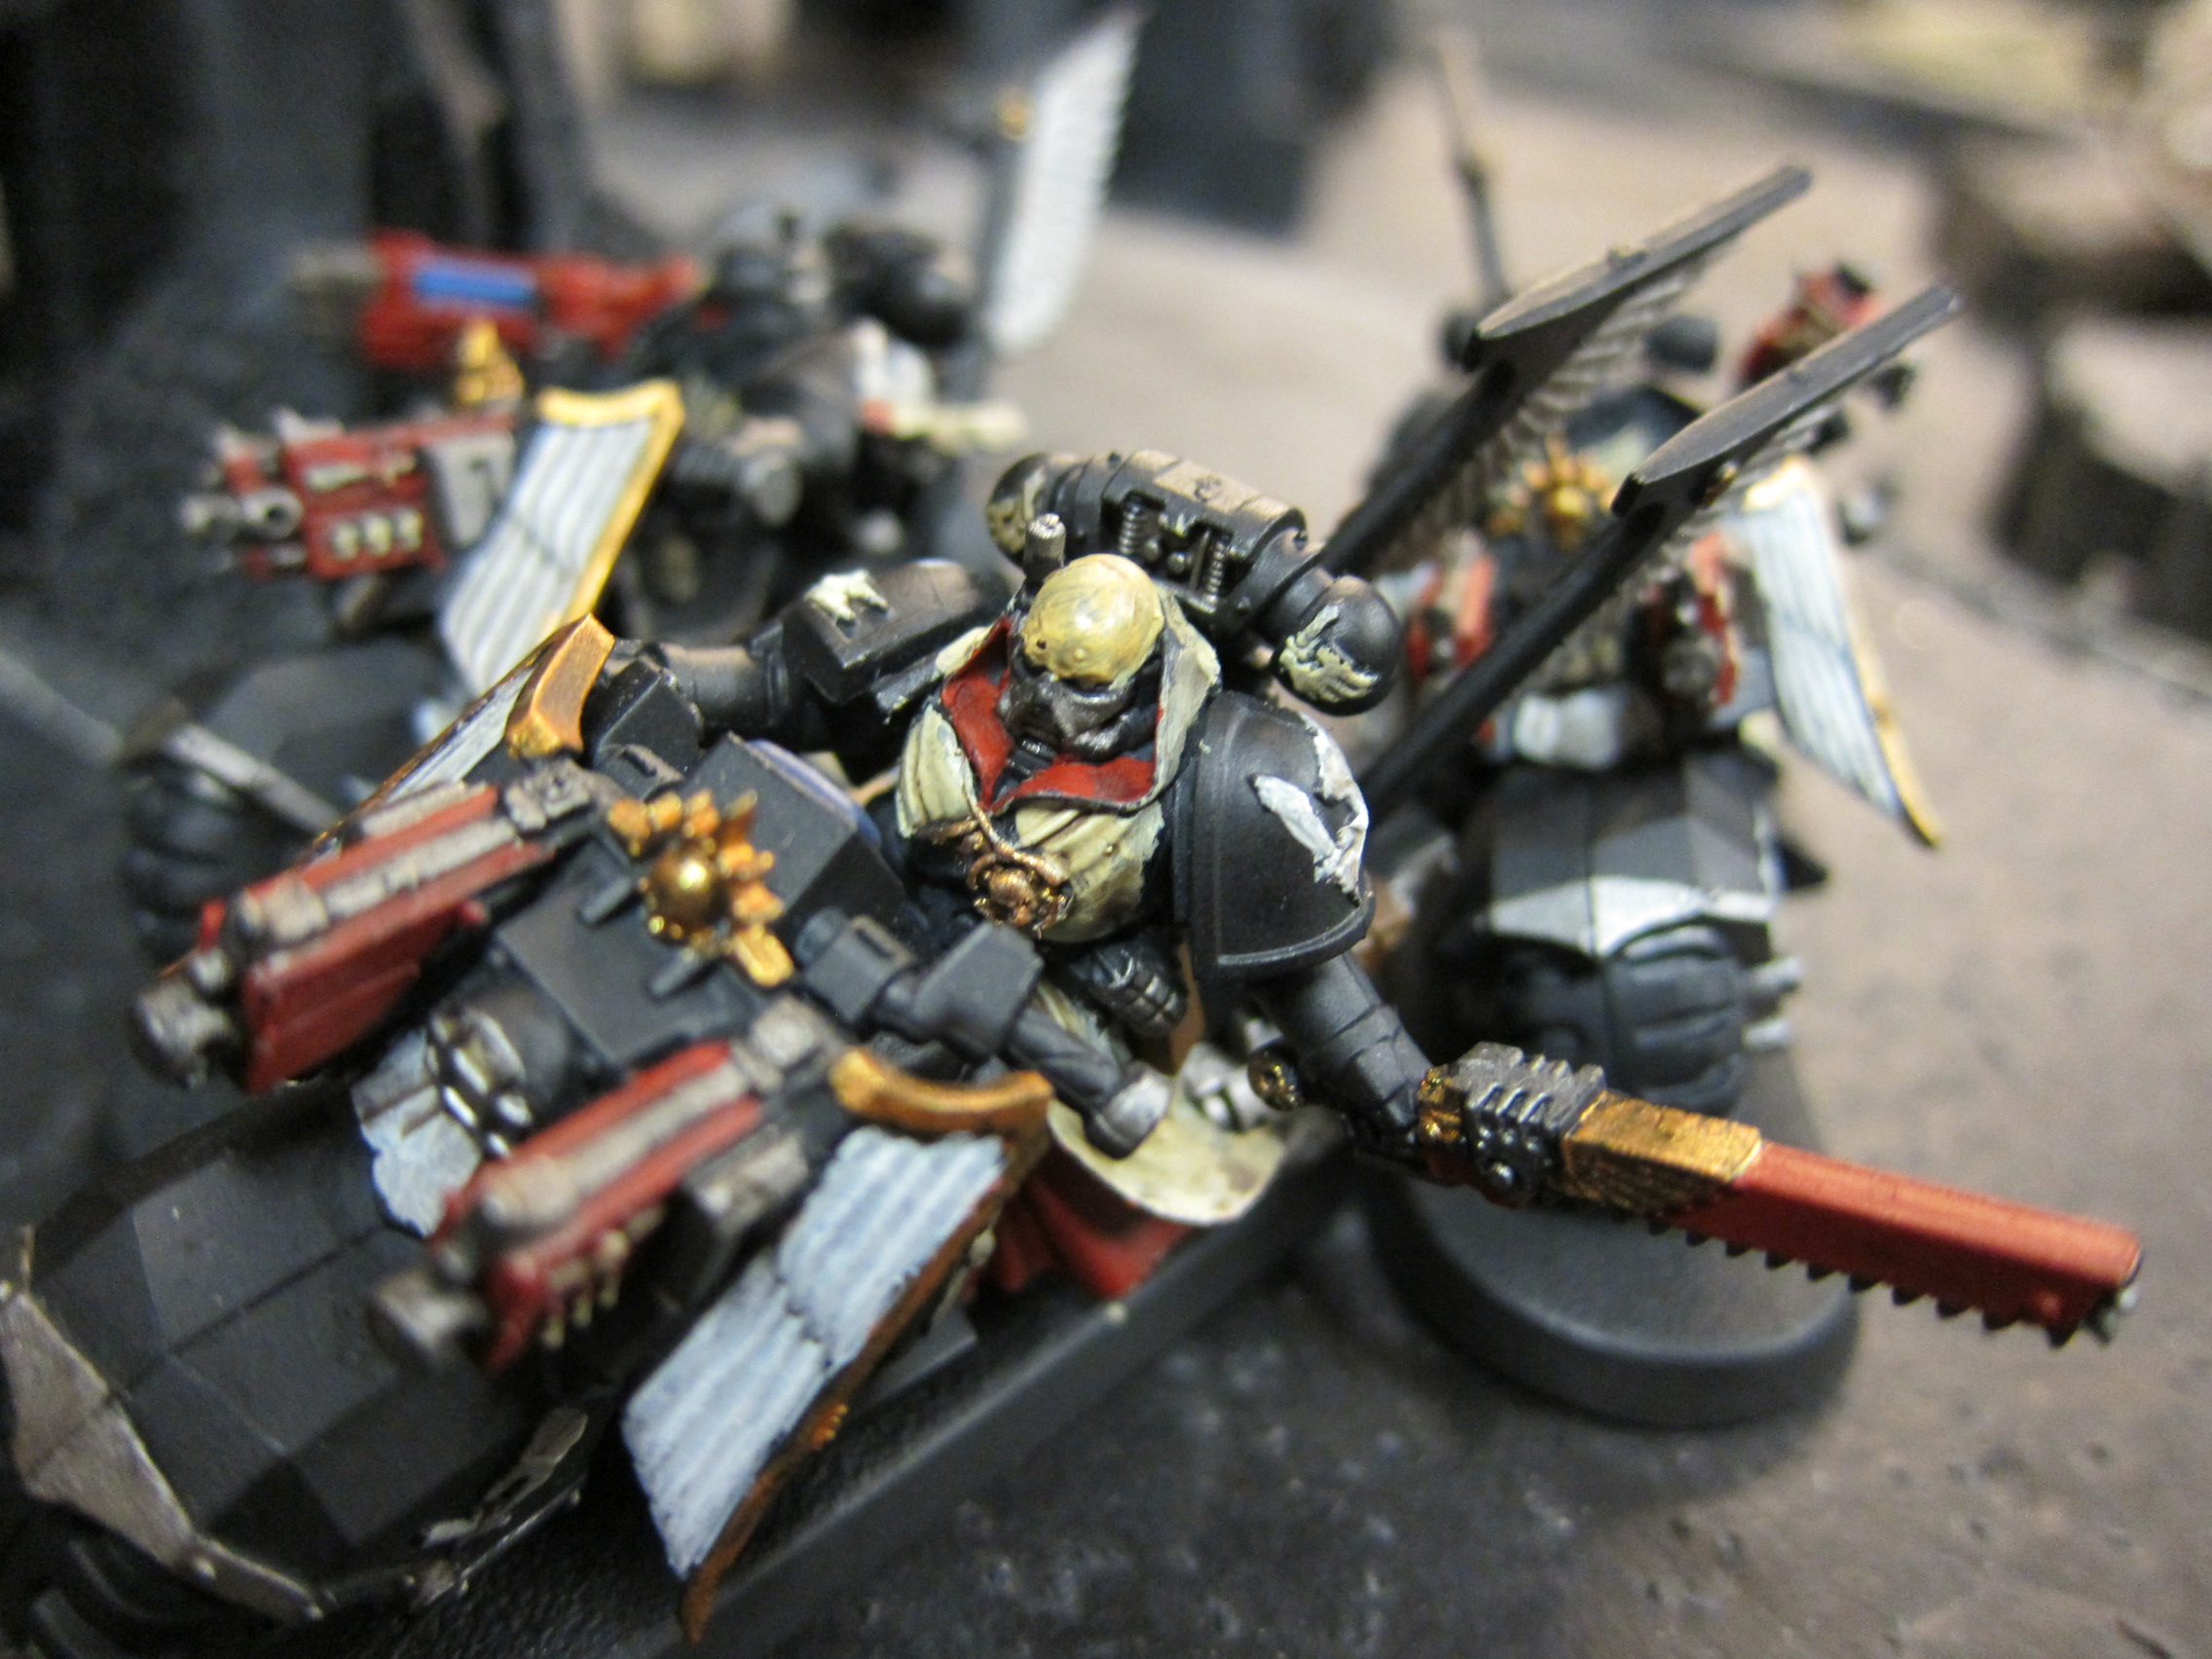
\includegraphics[width=(1.0\linewidth)]{pics/biker-sergeant}}\\
Cataclysm comes on our wings!
\end{minipage}
\vfill

%%------------------------------------------------------
\missionheading{Primary Objectives}%

The primary objective of the match is controlling important territory,
denoted by markers.  Primary objectives are placed after selecting
deployment zones.  First, each alliance in turn order places one home
objective in its deployment zone.  Each then in turn places one target
objective in the adjacent deployment zone clockwise around the table.
Finally, each alliance in turn then places one neutral objective on
the table in no alliance's deployment zone.  Objective marker
placement follows all standard rules.

After placing primary objective markers each alliance in turn order
deploys, using at most as many minutes as their deployment bid.  Units
not fully deployed at that point must be placed into reserve, except
for Infiltrators.  All other standard deployment and reserves rules
apply.


%%------------------------------------------------------
\missionheading{Game End \& Schedule}%

Cataclysm runs for a fixed~5 turns.  The organizer(s) should
enforce a schedule to ensure it finishes, such as that below for three
alliances.

Time must be reserved in each alliance turn for ongoing combats, lest
assault armies be short-changed.  These should begin to be resolved
with at least~5 minutes remaining in the turn.  Teammates already
finished their turn should help resolve ongoing combats if a player
engaged in an assault is still moving or shooting.  Otherwise the
engaged player must move on to assault with their turn unfinished.

\bigskip
\hrule
\vspace{2pt}
\centerline{\bf Cataclysm 3-Alliance Schedule}

\centerline{%
\begin{tabular}[t]{cl}
30 min & Set up tables \& terrain\\
45 min & Deployment \\
45 min & Turn 1 (15 min per alliance)\\
45 min & Turn 2\\
45 min & Turn 3\\
30 min & Turn 4 (10 min per alliance)\\
30 min & Turn 5\\
30 min & Pack up\\
\end{tabular}%
}
\hrule

%\vfill
%\bigskip
%\begin{story}{7pt}{Thought for the Day}
%Serve the Emperor, serve thyself.
%\end{story}
\pagebreak


%%------------------------------------------------------
\missionheading{Game Rules}%

\missionsubheading{Alliance Turns.}  Each player in an alliance
takes actions as usual in its turn, with any order of activated units.
Alliance turns are player turns in all ways.

\missionsubheading{Mission Rules.}  Standard nightfighting,
reserves, and objective control rules apply.

\missionsubheading{Table Scope.}  Special rules that affect all
units, all enemy units, or the entire table are not applied.

% Specific examples include the Chaos Daemons' Warp Storm table and the
% Lord of the Storm rules for the Necron's Imotekh the Stormlord as well
% as the Necron Solar Pulse, none of which take effect.

\missionsubheading{Army Scope.} Army-wide buffs apply only to that
detachment of that player's forces, as in a usual game, regardless of
factions in their alliance.

% E.g., fielding Vulkan makes only that player's Melta weapons in that
% detachment Mastercrafted and does not affect any detachment of other
% players in their alliance, including other Salamanders Space Marines.


\missionsubheading{Multi-Alliance Combats.} Units may charge as
usual into ongoing close combats including units from multiple other
alliances.  Combats are resolved in the assault phase of each alliance
with engaged units.

% making combats with more than two alliances particularly deadly!

\missionsubheading{Shooting at Combats.}  Players may shoot into
ongoing close combats that do not include any units from their
alliance.  Blast templates scatter as usual and hits are allocated to
units for each model under the template.  Other hits are allocated to
the unit of the model in the combat closest to each shooting model.

Regardless of the outcome, after resolving wounds the units in combat
are assumed to be still in combat unless all the models of an alliance
have been eliminated, even if models were removed such that the units
are no longer in contact.  Consolidation moves are not made if an
entire alliance is eliminated.  Units shot at in combat do not take
Morale Checks at the end of shooting, regardless of their casualties.

\missionsubheading{Psychic Phase.} A single D6 is rolled by the
current alliance to determine the base warp charge to be used by all
players in the psychic phase, who otherwise follow the standard rules
to generate their own distinct warp charge pools.  Players may only
cast and deny powers using their own warp charge.  The single player
from any opposing alliance willing to use the most warp charge to
attempt denying any successful spell may do so, breaking ties with a
roll-off.


% Each player generates and may only use their own warp charge pool,
% following the standard rules beyond that base charge.



%%------------------------------------------------------
\missionheading{Scoring}%

Primary objectives are cumulatively scored after
the~1st,~3rd, and~5th turns, the latter being the conclusion.  Their
worth to each alliance varies by location:

\begin{itemize}
\item Primary objectives in the next enemy deployment zone clockwise
  around the table are worth +3 victory points each.

\item Primary objectives in the alliance's own deployment zone are
  worth +2 victory points each.

\item All other primary objectives are worth +1 victory point each.
\end{itemize}

The following secondary objectives award additional victory points to
each alliance at game-end:
\begin{itemize}
\item +1 for each enemy warlord directly forced to be removed as a
  casualty by the alliance;

\item +1 for each enemy deployment zone in which the alliance has a
  scoring unit;

\item +1 if there are no enemy models, scoring or otherwise, in the
  alliance's own deployment zone.
\end{itemize}

The alliance with the most victory points emerges triumphant
from the Cataclysm!

\vfill
\noindent%
\begin{minipage}[h]{1.0\linewidth}\centering\small\it%
\fbox{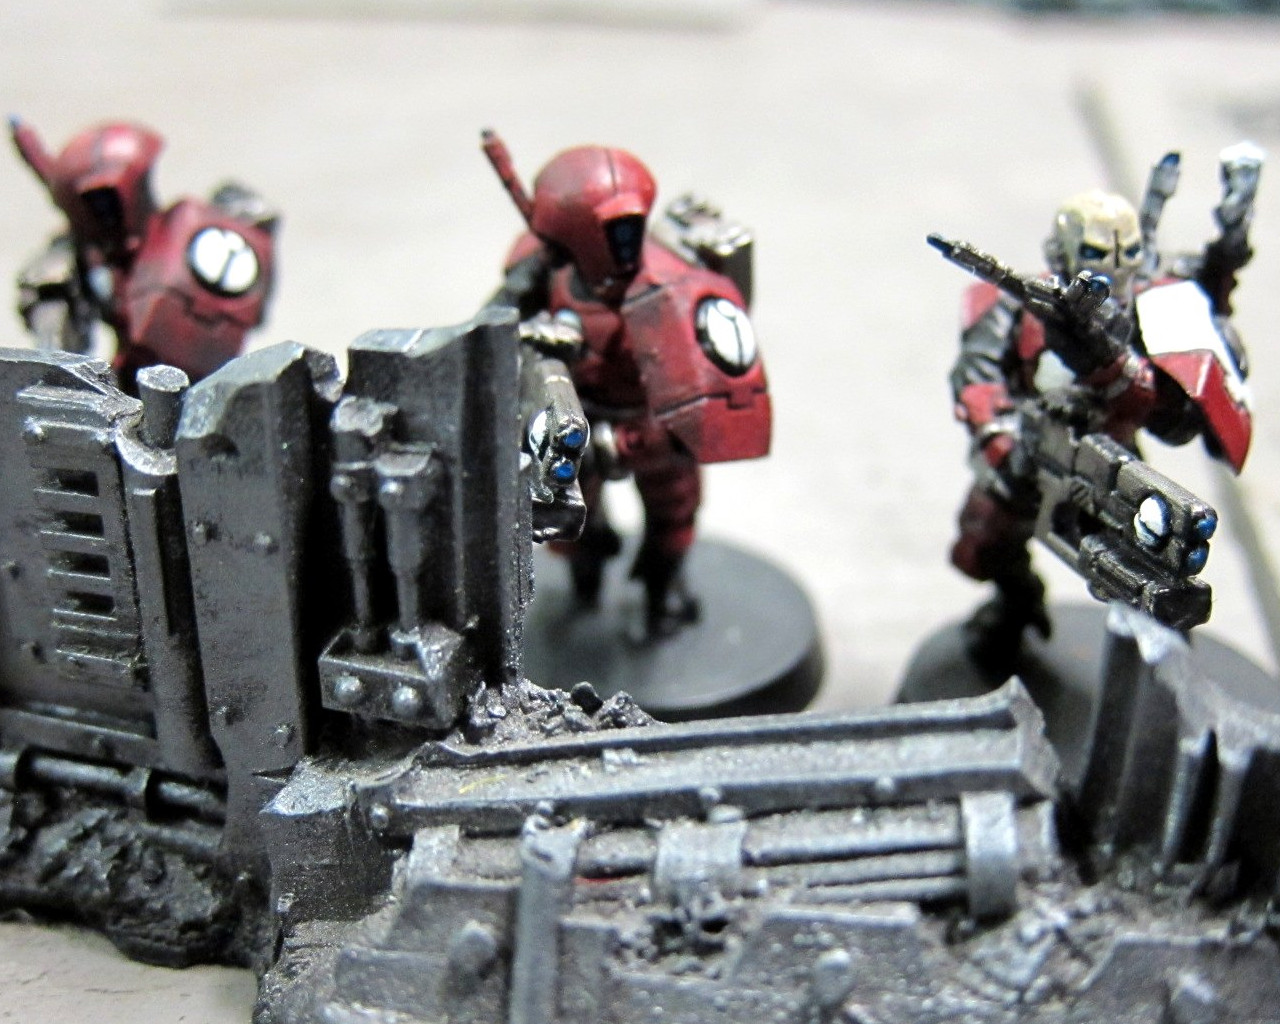
\includegraphics[width=(1.0\linewidth)]{pics/tau-line-cropped}}\\
Firing solution on coordinates alpha alpha nine six four!
\end{minipage}

\end{columns}

\vfill
\begin{story}{0.4in}{The Greater Good}
  Shas'ui Ke'ssai crouched low behind the crude rubble barricade.  His
  hooves trembled with the clamorous approach of the humans' ugly,
  stinking, smoking vehicles.  In that moment, he realized he hated
  them.  He hated them for their violence, and he hated them for what
  they'd done to his world.  But most of all, he hated them for
  teaching him to hate.
\end{story}



%%------------------------------------------------------
\pagebreak
\missionheading{Deployment Configurations}%

%%{\parfillskip0pt\relax\par}
\end{document}
